\documentclass[a4paper,11pt]{article}
\usepackage[utf8]{inputenc}
\usepackage[top=1.8cm,bottom=2.0cm,right=1.35cm,left=1.35cm]{geometry}
\usepackage{url}
\usepackage[natbibapa]{apacite}
\bibliographystyle{apacite}
\usepackage{graphicx}
\usepackage{amsmath}
\usepackage{amsfonts}
\usepackage{amssymb}
\usepackage[onehalfspacing]{setspace}
\usepackage{enumitem}
\usepackage{hyperref}
\usepackage{listings}
\usepackage{color}

\usepackage{lipsum}% this generates fictitious text for sample
%opening
\title{NewChic Dataset Analysis\\ Group 17}
\author{
    Karan Goel: SN 7836685\\
    Alvin Jose: SN 8066358 \\
    Ashutosh Bhosale: SN 7795786 \\
    Banin Sensha Shreshta: SN 8447196 \\
    Gaurav Adarsh Santosh: SN 7032663 \\
    Lino Thankachan: SN 7926017 \\
    Rishab Manokaran: SN 7863974 
}
\date{CSCI946 Big Data Analytics Assignment 1\\
August 23, 2024}

\begin{document}
\maketitle
\newpage
\section{Introduction}
\label{sec:introduction}

In the rapidly evolving e-commerce landscape, leveraging data is essential for making informed decisions regarding consumer behavior and business strategy. This report delves into an extensive analysis of the NewChic.com dataset, focusing on identifying the top 10 products from selected categories and determining the best-performing category.

Our approach began with data preparation and hypothesis testing to ensure accuracy and relevance. We employed two clustering algorithms—K-Means and Agglomerative Clustering (Hierarchical)—to uncover insights into customer behavior and preferences. By analyzing these clusters, we aimed to understand which products resonate most with consumers.

Furthermore, we utilized classification algorithms, including K-Nearest Neighbors and Decision Trees, to predict product popularity and assess the effectiveness of our model in forecasting trends.

This report provides a comprehensive overview of the data analysis process, highlighting the identification of best categories and top products. By comparing the performance of different clustering techniques, we offer actionable insights to enhance NewChic’s strategic decisions and optimize product offerings in the competitive e-commerce market.

\section{Task 1: Problem Analysis}

The dataset used in this analysis was compiled by merging nine different CSV files, each containing product data from distinct categories: accessories, bags, beauty, house, jewelry, kids, men, shoes, and women. This consolidation resulted in a comprehensive DataFrame consisting of 74,999 entries with 22 columns. For the purpose of this analysis, the focus was narrowed down to six key features:

\begin{itemize}
    \item \textbf{Category}: The type or category of the product (e.g., accessories, bags, etc.).
    \item \textbf{Name}: The specific name or identifier of the product.
    \item \textbf{Current Price}: The current selling price of the product.
    \item \textbf{Raw Price}: The original price of the product before any discounts.
    \item \textbf{Likes Count}: The number of likes or upvotes the product has received.
    \item \textbf{Discount}: The discount applied to the product, calculated as a percentage or fixed amount off the raw price.
\end{itemize}

\textbf{Objective:} The main objectives were to clean and prepare the data for analysis, explore the relationships between the selected features, and test specific hypotheses related to pricing, discounts, and customer preferences.

\subsection{Data Characteristics and Challenges}

The dataset presents several characteristics and challenges that must be addressed:

\begin{itemize}
    \item \textbf{Diversity of Categories}: The data spans nine distinct product categories, each likely to have different pricing structures, customer preferences, and discount strategies. This diversity requires careful handling during analysis to ensure meaningful comparisons and insights.
    \item \textbf{Size and Complexity}: With nearly 75,000 entries, the dataset is both large and complex, presenting potential computational challenges. Effective preprocessing and outlier detection are crucial to manage these complexities and ensure accurate analysis.
    \item \textbf{Missing Data}: Certain columns, particularly those related to \texttt{likes\_count} and \texttt{discount}, may contain missing values that need to be handled carefully to avoid biasing the analysis.
    \item \textbf{Outliers}: Given the range of products and categories, there may be significant outliers, particularly in numerical features such as \texttt{likes\_count} and \texttt{current\_price}. These outliers could skew the results if not properly managed.
    \item \textbf{Interdependencies Among Features}: Features such as \texttt{current\_price}, \texttt{raw\_price}, and \texttt{discount} are inherently related. Understanding these interdependencies is crucial for accurate analysis and hypothesis testing.
\end{itemize}

\subsection{Hypotheses and Analytical Focus}

Given the dataset's characteristics, the analysis focuses on the following key areas, each accompanied by formal hypotheses:

\begin{itemize}
    \item \textbf{Price Sensitivity and Customer Engagement}: Examining the relationship between \texttt{current\_price} and \texttt{likes\_count} to understand how price influences customer engagement.
    \begin{itemize}
        \item \textbf{Null Hypothesis (\( H_0 \))}: There is no significant correlation between the current price of a product and the number of likes it receives.
        \item \textbf{Alternative Hypothesis (\( H_A \))}: There is a significant correlation between the current price of a product and the number of likes it receives.
    \end{itemize}
    
    \item \textbf{Impact of Discounts}: Exploring how discounts affect \texttt{likes\_count} to uncover whether discounted products receive more attention.
    \begin{itemize}
        \item \textbf{Null Hypothesis (\( H_0 \))}: There is no significant relationship between the discount applied to a product and the number of likes it receives.
        \item \textbf{Alternative Hypothesis (\( H_A \))}: There is a significant relationship between the discount applied to a product and the number of likes it receives.
    \end{itemize}
    
    \item \textbf{Category-Specific Preferences}: Testing whether customer engagement, as measured by \texttt{likes\_count}, differs significantly across product categories.
    \begin{itemize}
        \item \textbf{Null Hypothesis (\( H_0 \))}: The average number of likes is the same across all product categories.
        \item \textbf{Alternative Hypothesis (\( H_A \))}: The average number of likes differs across at least one product category.
    \end{itemize}
\end{itemize}

These hypotheses guide the data preprocessing steps, ensuring that the dataset is prepared in a way that allows for robust and insightful analysis.

\section{Task 1: Data Preprocess}

The data preprocessing involved several critical steps to ensure the dataset was suitable for detailed analysis. Below is a breakdown of each step:

\subsection{Data Loading and Concatenation}

The first step was to load the nine CSV files into individual DataFrames and then concatenate them into a single unified DataFrame. This consolidation was essential for handling and analyzing the data as a cohesive unit.

\begin{lstlisting}[language=Python]
data_frames = {
    file.split('.')[0]: pd.read_csv(os.path.join(self.base_path, file))
    for file in self.files
}
self.df = pd.concat(data_frames.values(), ignore_index=True)
\end{lstlisting}

\subsection{Feature Selection and Handling Missing Values}

The next step involved selecting the six key features (category, name, current\_price, raw\_price, likes\_count, discount) and handling any missing values. Missing values in \texttt{likes\_count} and \texttt{discount} were filled with zeros, while missing values in \texttt{current\_price} were filled with the median value of that feature.

\begin{lstlisting}[language=Python]
chosen_columns = {
    'category', 'name', 'current_price', 'raw_price', 'likes_count', 'discount'
}
df = self.df.loc[:, self.df.columns.intersection(chosen_columns)]

fill_values = {
    'likes_count': 0,
    'discount': 0,
    'current_price': df['current_price'].median()
}
for column, value in fill_values.items():
    df[column] = df[column].fillna(value)
\end{lstlisting}

\subsection{Scaling Numerical Features}

To ensure that numerical features like \texttt{current\_price}, \texttt{raw\_price}, \texttt{discount}, and \texttt{likes\_count} were on a comparable scale, the \texttt{StandardScaler} was applied. This step standardizes the data, ensuring that each feature contributes equally to the analysis.

\begin{lstlisting}[language=Python]
numerical = df[['current_price', 'raw_price', 'discount', 'likes_count']]
scaled_features = self.scaler.fit_transform(numerical)
df[['current_price', 'raw_price', 'discount', 'likes_count']] = scaled_features
\end{lstlisting}

\subsection{Encoding Categorical Features}

Categorical features such as \texttt{category} and \texttt{name} were encoded using \texttt{LabelEncoder}. This step converted these features into numerical values, which are more suitable for machine learning models and statistical analysis.

\begin{lstlisting}[language=Python]
df['category'] = self.le_category.fit_transform(df['category'])
df['name'] = self.le_name.fit_transform(df['name'])
\end{lstlisting}

\subsection{Outlier Removal}

Outliers can skew analysis results, especially in a dataset with numerical features. Outliers were identified using the Z-score method, and any values exceeding the threshold of 3 were removed to ensure the dataset's integrity.

\begin{lstlisting}[language=Python]
z_scores = np.abs(stats.zscore(df.select_dtypes(include=[np.number])))
inliers = (z_scores < 3).all(axis=1)
df = df[inliers]
\end{lstlisting}

\subsection{Task 1: Results}

To test Hypotheses 1 and 2, we first constructed a correlation matrix and computed the corresponding p-values, using a significance level (\(\alpha\)) of 0.05 Figure \ref{fig:corr}. Additionally, to address Hypothesis 3, we performed an ANOVA test to determine if the average \texttt{likes\_count} varies across product categories. Figure \ref{fig:box}

\begin{figure}[h!]
    \centering
    \begin{minipage}{0.45\textwidth}
        \centering
        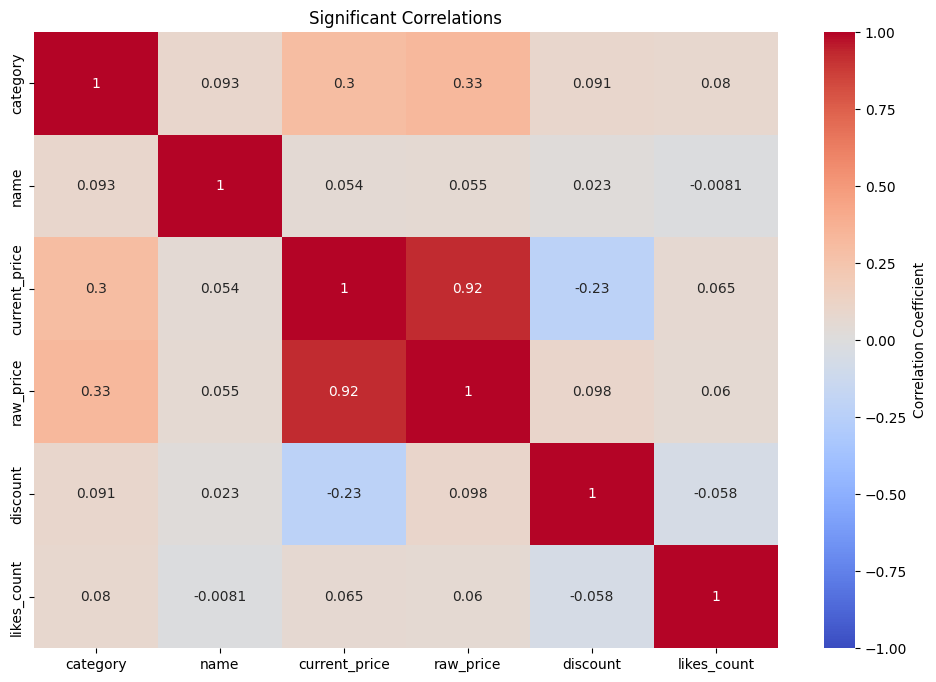
\includegraphics[width=\textwidth]{corr.png}
        \caption{Correlation Matrix}
        \label{fig:corr}
    \end{minipage}
    \hfill
    \begin{minipage}{0.45\textwidth}
        \centering
        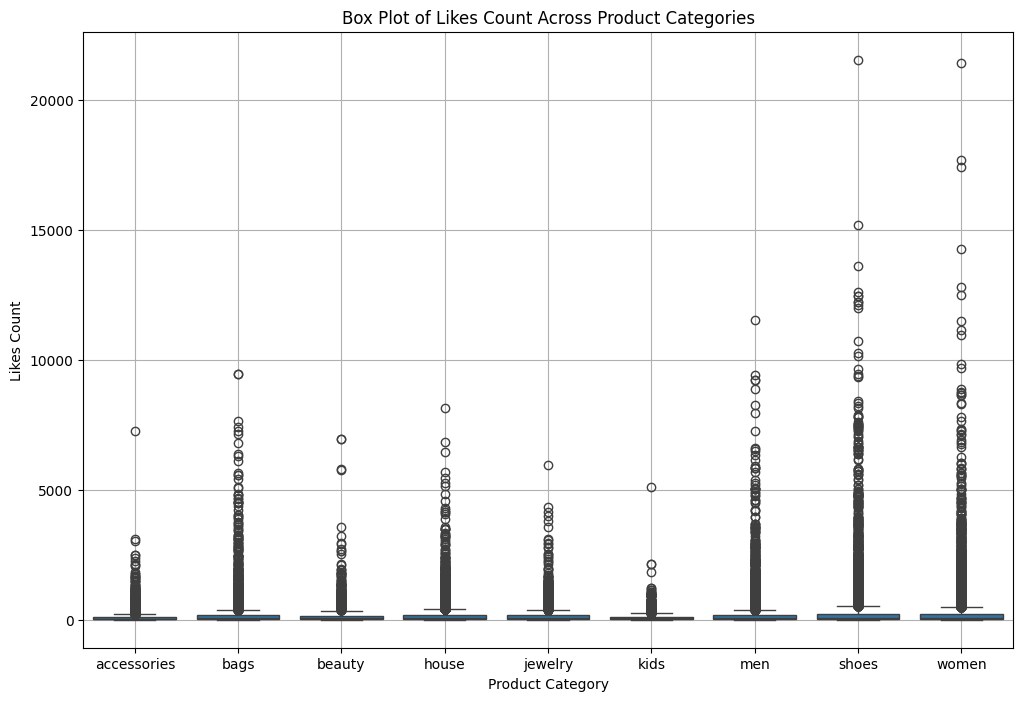
\includegraphics[width=\textwidth]{box.png}
        \caption{Box Chart for Categories}
        \label{fig:box}
    \end{minipage}
\end{figure}

\textbf{Results:} In both cases, we rejected the null hypotheses.

Based on these findings, we identified the top 7 categories and top 10 products by evaluating \texttt{likes\_count}, \texttt{current\_price}, and \texttt{discount}.

Detailed results are provided in Section \ref{sec:result}.


\section{Task 2: Clustering}

Our objective is to cluster customer preferences to determine the types of products that are most favored by different customer segments. We proceed as follows:

\begin{itemize}
\item \textbf{Feature Selection}: The analysis focused on the current\_price and discount columns. The raw\_price and likes\_count columns were excluded as they were not necessary for the clustering process.
\item \textbf{Target Data}: The name and category columns were retained as target data. Although these columns were not used directly for clustering, they were later employed for interpreting the resulting clusters.
\end{itemize}


\subsection{Elbow Method}

The Elbow Method was employed to determine the optimal number of clusters for the KMeans algorithm. This method involves plotting the Within-Cluster Sum of Squares (WSS) against the number of clusters to identify the "elbow point," which indicates the number of clusters beyond which adding more clusters does not significantly reduce the WSS. Figure \ref{fig:wss}

\begin{figure}[h!]
    \centering
    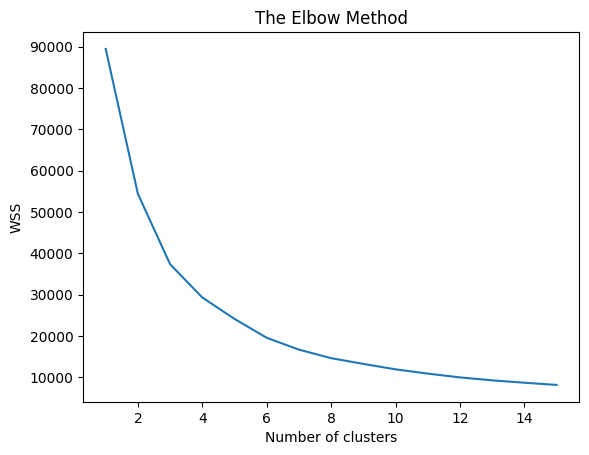
\includegraphics[width=0.7\textwidth]{wss.png}
    \caption{WSS}
    \label{fig:wss}
\end{figure}

Based on this method, we determined the optimal value for k to be \textbf{7}.

\subsection{Clustering Algorithms}

Two clustering algorithms were employed:

\begin{itemize}
    \item \textbf{KMeans}: A centroid-based clustering algorithm that partitions the dataset into $k$ clusters, with each cluster represented by the mean of the points within it.
    \item \textbf{Agglomerative Clustering}: A hierarchical clustering technique that builds nested clusters by merging or splitting them successively.
\end{itemize}

Both algorithms were executed with $k=7$ clusters, and the results were evaluated using the following metrics:

\begin{itemize}
    \item \textbf{Silhouette Score}: Measures how similar an object is to its own cluster compared to other clusters.
    \item \textbf{Calinski-Harabasz Index}: The ratio of the sum of between-clusters dispersion and within-cluster dispersion.
    \item \textbf{Davies-Bouldin Index}: The average similarity ratio of each cluster with its most similar cluster.
\end{itemize}

The clustering process is implemented as follows:

\begin{lstlisting}[language=Python]
def perform_clustering(self):
    algorithms = {
        "KMeans": KMeans(n_clusters=7, max_iter=1000),
        "Agglomerative": AgglomerativeClustering(n_clusters=7, linkage='ward')
    }

    for name, algorithm in algorithms.items():
        labels = algorithm.fit_predict(self.X)
        
        # Store the calculated metrics
        self.metrics["Silhouette Score"][name] = silhouette_score(
            self.X, labels)
        self.metrics["Calinski-Harabasz Index"][name] = calinski_harabasz_score(
            self.X, labels)
        self.metrics["Davies-Bouldin Index"][name] = davies_bouldin_score(
            self.X, labels)
\end{lstlisting}

\subsection{Visualization}

Clusters were visualized by plotting the `current\_price` against the `discount` and coloring the points based on their cluster assignments. Additionally, top products were highlighted in red to emphasize their positioning within the clusters. Figure \ref{fig:kmean} and \ref{fig:algo}

This helped us understand customer preferences regarding pricing and discounts.

\begin{figure}[h!]
    \centering
    \begin{minipage}{\textwidth}
        \centering
        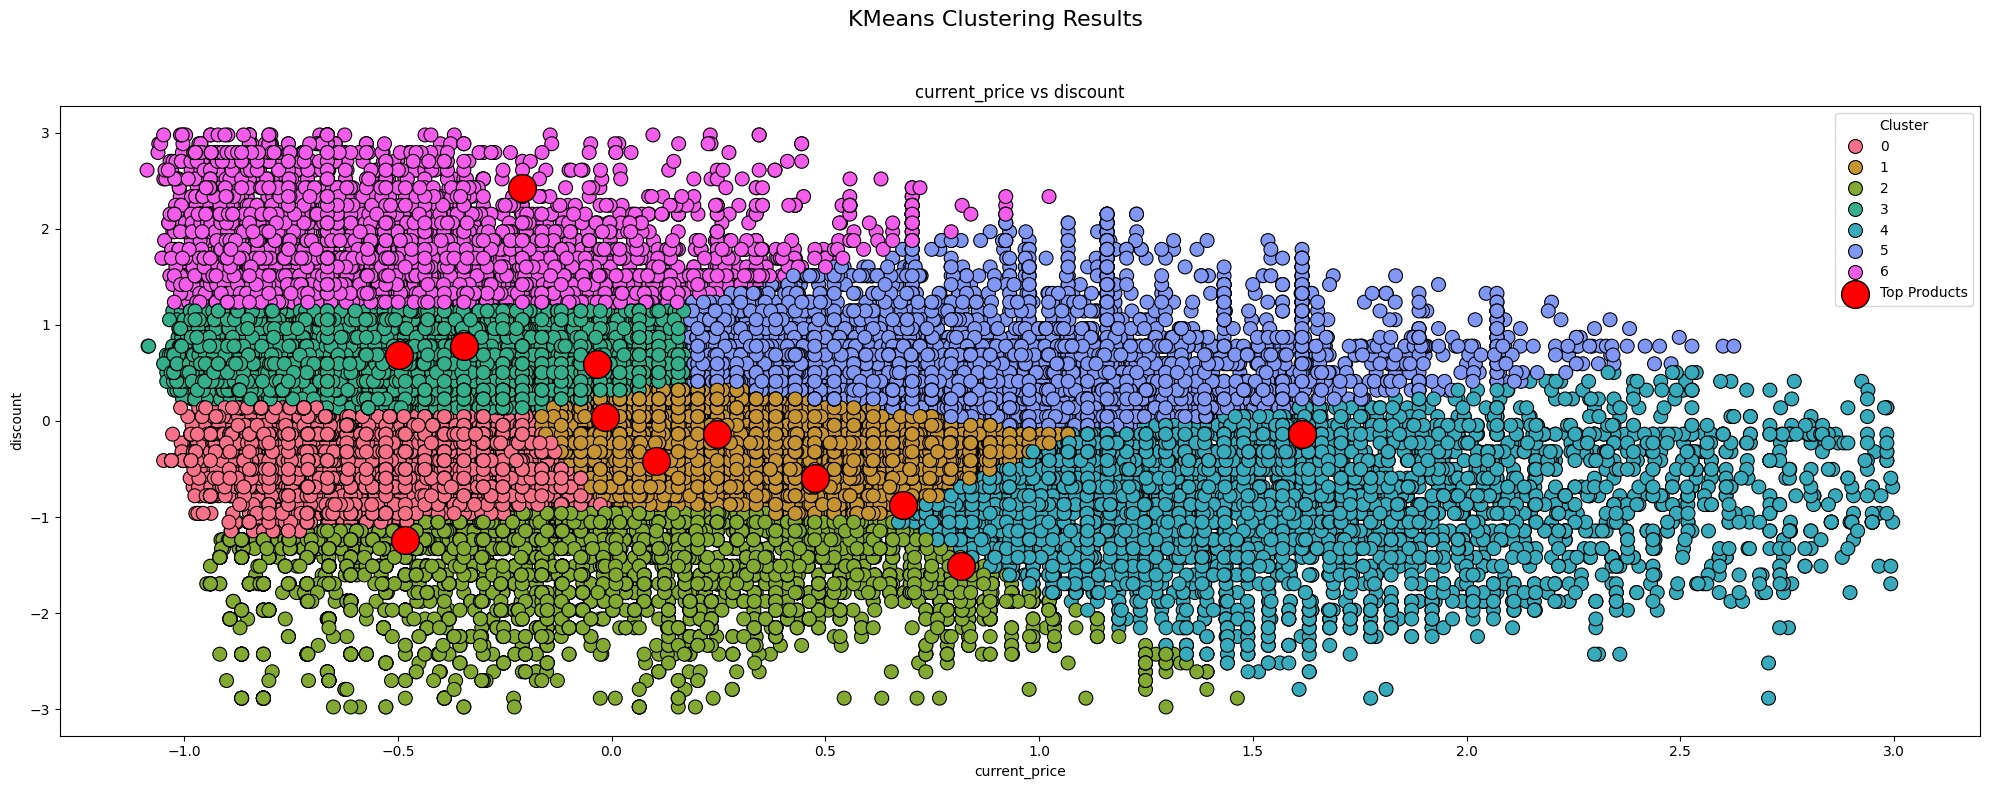
\includegraphics[width=\textwidth]{kmeans.png}
        \caption{Kmeans Cluster}
        \label{fig:kmean}
    \end{minipage}
    \hfill
    \begin{minipage}{\textwidth}
        \centering
        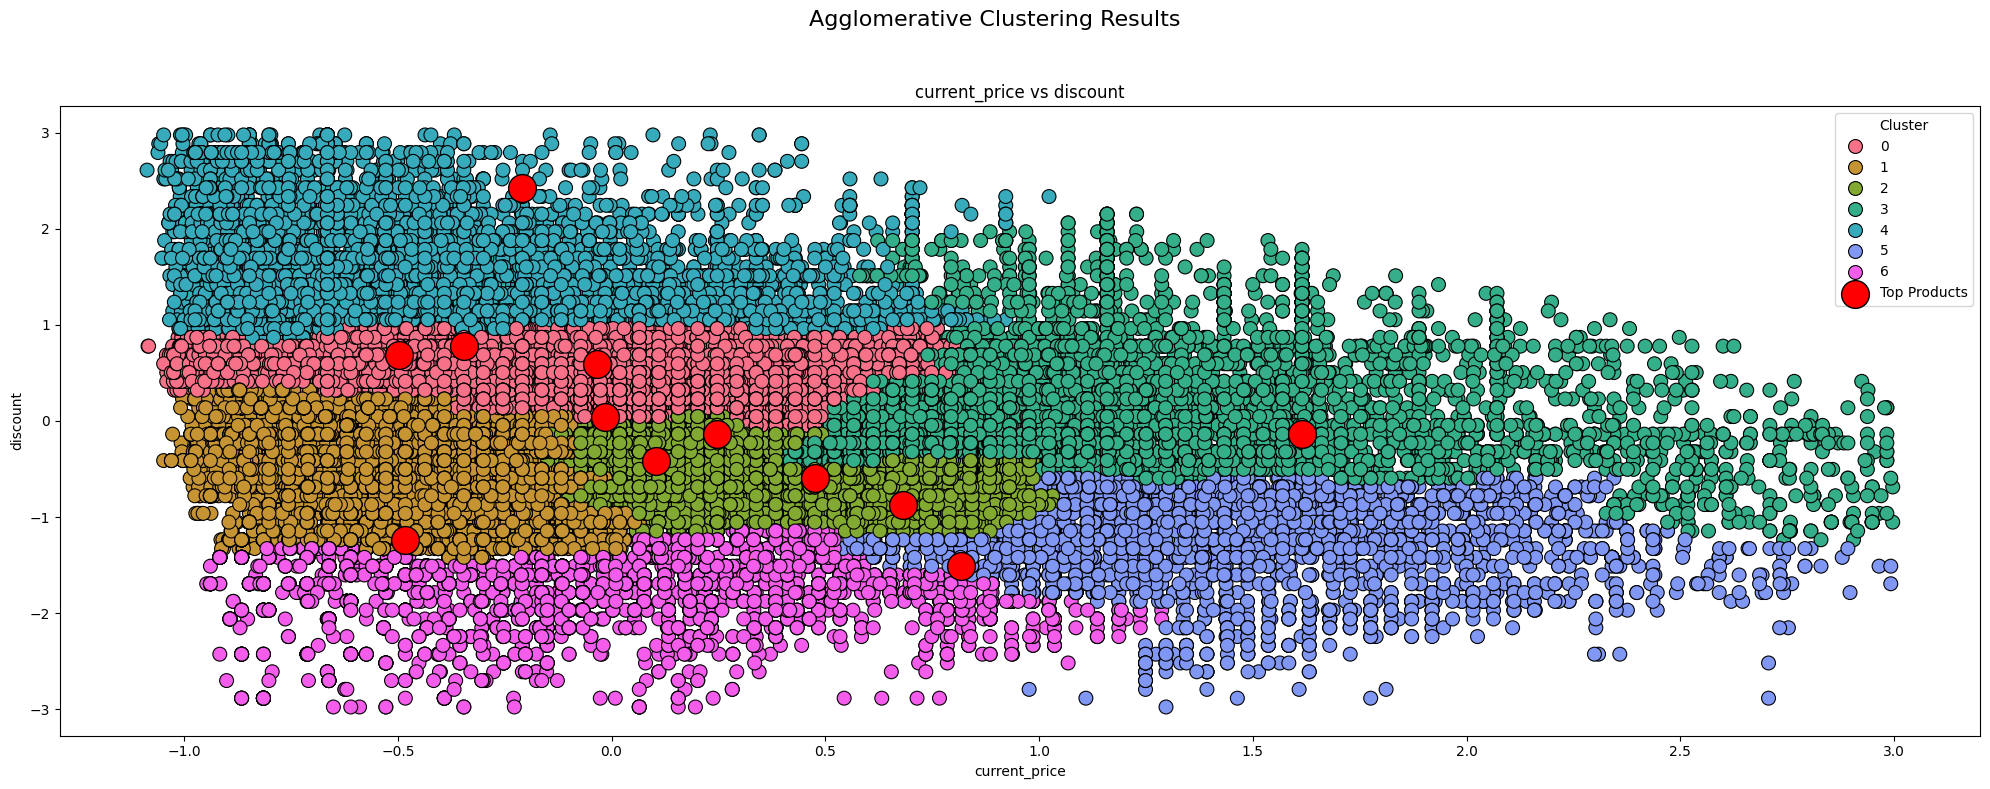
\includegraphics[width=\textwidth]{algo.png}
        \caption{Hierarchy Clusters}
        \label{fig:algo}
    \end{minipage}
\end{figure}

\subsection{Justification and Selection of Algorithms}
\begin{itemize}
    \item \textbf{KMeans Clustering:} 
    \begin{itemize}
        \item \textbf{Reason for Selection:} KMeans is efficient for large datasets and partitions data into `K` clusters based on proximity to the cluster mean.
        \item \textbf{Strengths:} Computationally faster, works well with spherical clusters, easy to implement and interpret.
        \item \textbf{Weaknesses:} Requires pre-specification of `K`, struggles with non-spherical clusters.
    \end{itemize}
    \item \textbf{Agglomerative Clustering:}
    \begin{itemize}
        \item \textbf{Reason for Selection:} Hierarchical technique capturing complex relationships, useful for understanding data structure.
        \item \textbf{Strengths:} Does not require pre-specification of clusters, can visualize clustering with a dendrogram.
        \item \textbf{Weaknesses:} Computationally expensive, less effective for large datasets.
    \end{itemize}
\end{itemize}

\subsection{Task 2: Results}

This clustering analysis successfully grouped similar products based on their current price and discount. The KMeans algorithm, with $k=7$ clusters, demonstrated the best performance according to the Silhouette Score, although both algorithms provided valuable insights. The visualizations highlighted the distribution of clusters and the positioning of top products, offering a clear view of the clustering results.


\begin{table}[h!]
\centering
\begin{tabular}{|c|c|c|c|}
\hline
\textbf{Algorithm} & \textbf{Silhouette Score} & \textbf{Calinski-Harabasz Index} & \textbf{Davies-Bouldin Index} \\ \hline
KMeans             & 0.4281                    & 48062.9940                       & 0.7600                        \\ \hline
Agglomerative      & 0.3829                    & 20383.9248                       & 0.8066                        \\ \hline
\end{tabular}
\caption{Comparison of Clustering Algorithms}
\end{table}

\section{Task 3: Classification}

Our objective for the classification task is to predict the popularity of a product based on its current price, discount, and category. We employed two different machine learning algorithms: K-Nearest Neighbors (KNN) and Decision Trees.

\subsection{Data Preprocessing}

To prepare the data for classification, the following steps were undertaken:

\begin{enumerate}
    \item \textbf{Popularity Definition}: A new binary target variable, \textit{popularity}, was created based on the \textit{likes\_count} feature. Products with a \textit{likes\_count} higher than the dataset's mean were classified as popular (\texttt{popularity = 1}), and the rest as not popular (\texttt{popularity = 0}).
    \item \textbf{Feature Selection}: The features selected for the classification task included \textit{category}, \textit{current price}, and \textit{discount}. The target variable was \textit{popularity}.
    \item \textbf{Train-Test Split}: The dataset was split into training and testing sets, with 80\% of the data used for training and 20\% reserved for testing.
\end{enumerate}

\subsection{K-Nearest Neighbors (KNN)}

\subsubsection{Algorithm Overview}

K-Nearest Neighbors (KNN) is a simple, instance-based learning algorithm that classifies a data point based on the majority class of its \(k\) nearest neighbors in the feature space. The choice of \(k\) is critical; a smaller \(k\) can lead to high variance, while a larger \(k\) may increase bias.

The KNN model was trained using a range of odd values for \(k\) between 13 and 19, with the Manhattan distance metric. The best parameters were selected through GridSearchCV, optimizing for accuracy.

\begin{lstlisting}[language=Python]
    def train_knn(self):
        knn = KNeighborsClassifier()
        param_grid = {
            'n_neighbors': [i for i in range(13, 20, 2)],
            'weights': ['uniform'],
            'metric': ['manhattan']
        }
        grid_search = GridSearchCV(
            knn, param_grid, cv=self.skf, scoring='accuracy')
        grid_search.fit(self.X_train, self.y_train)

        # Best KNN model
        self.knn_model = grid_search.best_estimator_
        print(f"Best KNN Parameters: {grid_search.best_params_}")

        # Cross-validation scores
        cv_scores = cross_val_score(
            self.knn_model, self.X_train, self.y_train, cv=self.skf, scoring='accuracy')
        print(f'KNN Average Accuracy: {cv_scores.mean()
\end{lstlisting}

\subsection{Decision Tree}

\subsubsection{Algorithm Overview}

A Decision Tree is a supervised learning algorithm that splits the dataset into subsets based on feature values, creating a tree-like structure of decisions. Each internal node of the tree represents a decision based on a feature, each branch represents the outcome of that decision, and each leaf node represents a class label or regression value. Decision Trees can be used for both classification and regression tasks.

Key parameters for Decision Trees include:
\begin{itemize}
    \item \textbf{Criterion}: The function used to measure the quality of a split (e.g., Gini impurity, entropy).
    \item \textbf{Max Depth}: The maximum depth of the tree, controlling the complexity and preventing overfitting.
    \item \textbf{Min Samples Split}: The minimum number of samples required to split an internal node.
    \item \textbf{Min Samples Leaf}: The minimum number of samples required to be at a leaf node.
\end{itemize}

The following Python code demonstrates the implementation of the KNN and Decision Tree algorithms for classifying product popularity.

\begin{lstlisting}[language=Python] 
    def train_decision_tree(self):
        print("Decision Tree")
        dt = DecisionTreeClassifier(random_state=42)
        param_grid = {
            'criterion': ['gini', 'entropy'],
            'max_depth': [None, 10, 20, 30, 40, 50],
            'min_samples_split': [2, 5, 10, 15],
            'min_samples_leaf': [1, 2, 4, 6]
        }
        grid_search = GridSearchCV(
            dt, param_grid, cv=self.skf, n_jobs=-1, verbose=2)
        grid_search.fit(self.X_train, self.y_train)

        # Best Decision Tree model
        self.dt_model = grid_search.best_estimator_
        print(f"Best Decision Tree Parameters: {grid_search.best_params_}")

        # Cross-validation scores
        cv_scores = cross_val_score(
            self.dt_model, self.X_train, self.y_train, cv=self.skf, scoring='accuracy')
        print(f'Decision Tree Average Accuracy: {cv_scores.mean() * 100:.2f}%')
        print(f'Decision Tree Standard Deviation: {cv_scores.std() * 100:.2f}%')
\end{lstlisting}

\subsection{Justification and Selection of Algorithms}
\begin{itemize}
    \item \textbf{K-Nearest Neighbors (KNN):}
    \begin{itemize}
        \item \textbf{Reason for Selection:} KNN is a straightforward and intuitive algorithm that works well for classification tasks where decision boundaries are not linear.
        \item \textbf{Strengths:}
        \begin{itemize}
            \item \textbf{Simplicity:} Easy to implement and understand.
            \item \textbf{Flexibility:} Can be used for both classification and regression.
            \item \textbf{No Assumptions:} Makes no assumptions about the underlying data distribution.
            \item \textbf{Adaptability:} Effective with small to medium-sized datasets.
        \end{itemize}
    \end{itemize}
    \item \textbf{Decision Trees:}
    \begin{itemize}
        \item \textbf{Reason for Selection:} Decision Trees are chosen for their interpretability and ability to handle non-linear relationships in the data.
        \item \textbf{Strengths:}
        \begin{itemize}
            \item \textbf{Interpretability:} Easy to interpret and visualize, allowing us to understand the decision-making process and the importance of different features.
            \item \textbf{Non-Linear Relationships:} Can capture complex, non-linear relationships between features and the target variable.
            \item \textbf{Feature Importance:} Provides insights into which features contribute most to the predictions.
            \item \textbf{No Need for Feature Scaling:} Does not require feature scaling, simplifying preprocessing.
            \item \textbf{Handling of Missing Values:} Can handle missing values in the dataset, making them robust to incomplete data.
            \item \textbf{Versatility:} Suitable for both classification and regression tasks.
        \end{itemize}
    \end{itemize}
\end{itemize}

\subsection{Task 3: Results}

Both algorithms achieved an accuracy of 77\% on the dataset, with good precision, recall, and F1 scores. The Decision Tree performed slightly better than K-Nearest Neighbors.

\begin{figure}[h!]
    \centering
    \begin{minipage}{0.45\textwidth}
        \centering
        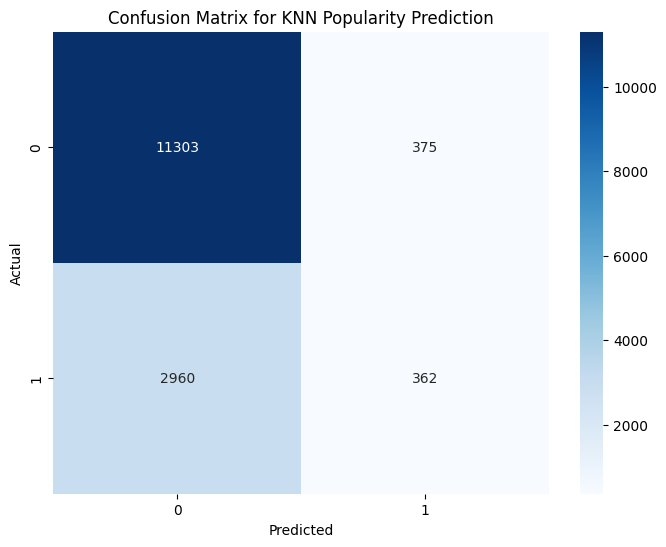
\includegraphics[width=\textwidth]{knn.png}
        \caption{Confusion Matrix for K-Nearest Neighbors}
        \label{fig:knn}
    \end{minipage}
    \hfill
    \begin{minipage}{0.45\textwidth}
        \centering
        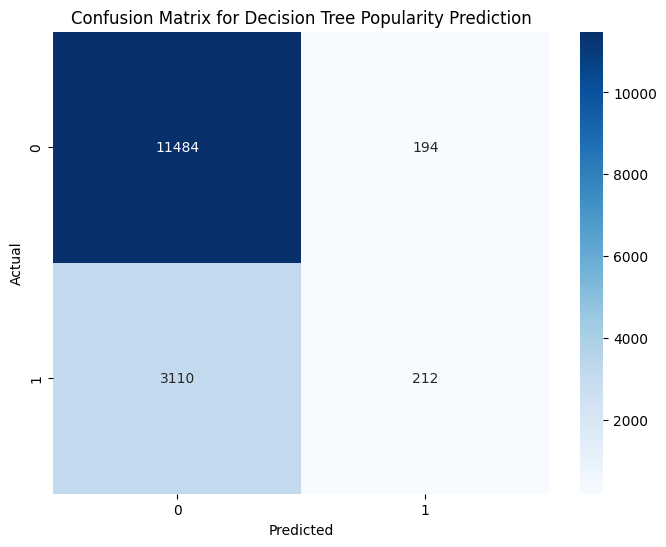
\includegraphics[width=\textwidth]{dt.png}
        \caption{Confusion Matrix for Decision Tree}
        \label{fig:dt}
    \end{minipage}
\end{figure}

\begin{figure}[h!]
    \centering
    \begin{minipage}{0.45\textwidth}
        \centering
        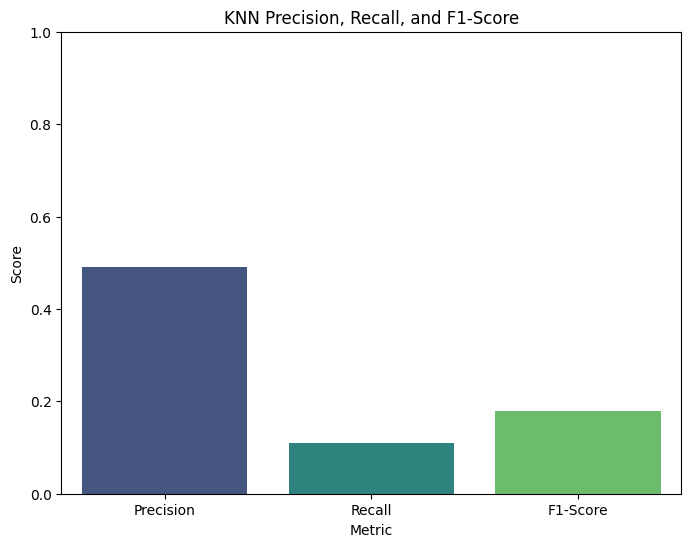
\includegraphics[width=\textwidth]{knn1.png}
        \caption{Performance Metrics for K-Nearest Neighbors}
        \label{fig:knn1}
    \end{minipage}
    \hfill
    \begin{minipage}{0.45\textwidth}
        \centering
        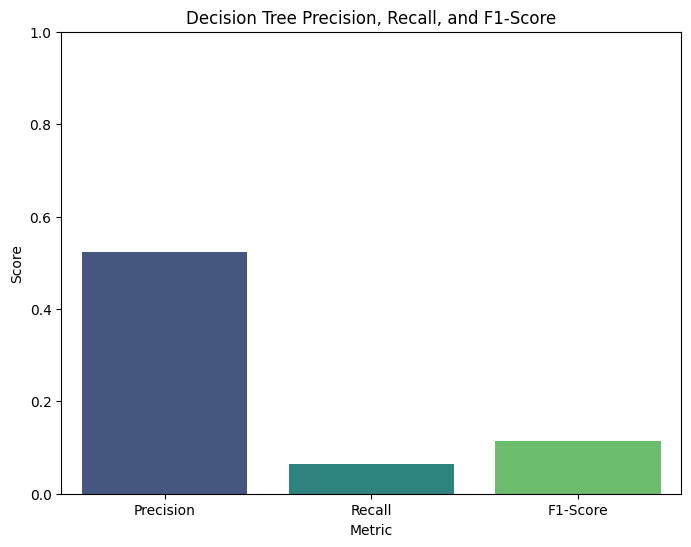
\includegraphics[width=\textwidth]{dt1.png}
        \caption{Performance Metrics for Decision Tree}
        \label{fig:dt1}
    \end{minipage}
\end{figure}

\section{Task 4: Result Discussion}
\label{sec:result}

\subsection{Are the clusters well-separated from each other?}

\noindent
The clusters are indeed well-separated. We determined the optimal number of clusters \( k \) to be 7 by using the Within-Cluster Sum of Squares (WSS) criterion. Plotting the clusters against features such as discount and current price clearly shows distinct separations between clusters. This indicates that the clustering process has effectively identified separate groups within the data.

\subsection{ Did the classifiers separate products into different classes effectively?}

\noindent
The classifiers demonstrated competent performance in distinguishing products into different classes. The K-Nearest Neighbors (KNN) classifier achieved an accuracy of 77\%, while the Decision Trees classifier achieved a slightly higher accuracy of 78\%. Further analysis revealed that Decision Trees outperformed KNN in terms of Precision, Recall, and F1 Score, suggesting that Decision Trees provide a more balanced classification performance in this context.

\subsection{Do any of the clusters/classes have only a few points?}

\noindent
No, all clusters contain a sufficient number of data points. The distribution across clusters is balanced, with none of the clusters having a disproportionately small number of points. This implies that the data is well-represented across all clusters, contributing to the robustness of the analysis.

\subsection{Are there meaningful and non-meaningful clusters/classes with respect to the analytics problems outlined in Task 1?}

\noindent
\textbf{Meaningful Clusters:} The analysis reveals that clusters containing products with low current prices, even in the absence of significant discounts, tend to include well-liked products. This suggests that price is a key factor in customer preference, providing actionable insights into pricing strategies.

\noindent
\textbf{Non-Meaningful Clusters:} Some clusters encompass information from various categories without a clear pattern or insight. These clusters do not provide specific actionable information and may reflect a more random distribution of product attributes.

\subsection{What are the advantages and shortcomings of clustering and classification algorithms in this analytics case? Which algorithm provides more valuable results?}

\noindent
\textbf{Clustering (K-Means):}
\begin{itemize}
    \item \textbf{Advantages:} Effective at identifying natural groupings within the data and requires relatively few computational resources. Useful for segmenting products based on attributes like price and discount.
    \item \textbf{Shortcomings:} Sensitive to the initial placement of cluster centroids and the scaling of data. It may not perform well with outliers and requires the number of clusters to be specified in advance.
\end{itemize}

\noindent
\textbf{Classification (KNN and Decision Trees):}
\begin{itemize}
    \item \textbf{Advantages:} KNN is effective at capturing local patterns, while Decision Trees offer interpretability and can handle complex relationships in the data. Both models provide insights into how features like price and discount influence product classification.
    \item \textbf{Shortcomings:} KNN can be computationally expensive with large datasets, and Decision Trees may overfit if not properly tuned. The performance of KNN may degrade with increased dataset size.
\end{itemize}

\noindent
\textbf{Which Algorithm Provides Greater Value:} In this case, K-Means clustering was particularly valuable as it provided insights into customer behavior and product segmentation. Although Decision Trees performed better in classification tasks, the computational expense of KNN and the interpretability of Decision Trees suggest that clustering offered more actionable insights for understanding product groupings and pricing strategies.

\subsection{Are the examined algorithms suitable for Big Data analytics? If so, why?}

\noindent
\textbf{K-Means Clustering:} K-Means is suitable for large datasets due to its relatively low computational complexity. However, with very large datasets, it may become computationally intensive and sensitive to high-dimensional data. 

\noindent
\textbf{KNN:} KNN is generally not well-suited for Big Data analytics because it requires storing the entire training dataset and has high computational costs, especially for large datasets.

\noindent
\textbf{Decision Trees:} Decision Trees are more scalable and can handle larger datasets better than KNN. They are effective in managing complexity and high-dimensional data, though they may require careful tuning to avoid overfitting with very large datasets.

\subsection{Will data preprocessing affect clustering and classification results? If so, how?}

\noindent
Yes, data preprocessing significantly impacts both clustering and classification results. 
\begin{itemize}
    \item \textbf{Scaling:} Standardizing or normalizing data ensures that all features contribute equally to distance calculations, which is crucial for algorithms like K-Means and KNN.
    \item \textbf{Outliers:} Removing outliers enhances the robustness of clustering and classification algorithms, preventing them from being unduly influenced by extreme values.
\end{itemize}
Proper preprocessing improves the quality of the clusters and the accuracy of the classifiers by ensuring that the data is clean, well-scaled, and appropriately prepared for analysis.



% Table 1: Top Categories
\begin{table}[h!]
    \centering
    \caption{Top 7 Categories (based on average likes count)}
    \begin{tabular}{|l|}
        \hline
        \textbf{Category} \\
        \hline
        Shoes \\
        Women \\
        Jewelry \\
        House \\
        Bags \\
        Men \\
        Beauty \\
        \hline
    \end{tabular}
\end{table}

% Table 2: Top Products in the Top 7 Categories
\begin{table}[h!]
    \centering
    \caption{Top 10 Products in the Top 7 Categories}
    \begin{tabular}{|l|}
        \hline
        \textbf{Product} \\
        \hline
        Sandales élastiques à strass perle \\
        Chaussures Vintage Rétro Respirantes Maille Ballerines À Fleur Avec Noeud Chinois \\
        Sac de rangement étanche \\
        Combinaison ample sans manches \\
        Tongs plats en suède à entredoigt à fleur décorative \\
        Bottes Vintage à Imprimé Fleurs \\
        Manteau à Capuche Imprimé avec Poches \\
        12 couleurs maquillage ombre à paupières stylo \\
        Pompes papillon peintes à la main \\
        Robe Casual Couleur Unie \\
        \hline
    \end{tabular}
\end{table}

\newpage
\bibliography{bibliography_data}
\nocite{*}
\end{document}
